\chapter{Analyse et spécification des besoins}
\label{chap:analyse-besoins}

Ce chapitre traduit les constats du chapitre précédent en besoins précis. Pour le \ac{CTAA}, nous identifions les acteurs du \ac{LIMS}, formulons ses besoins fonctionnels et non fonctionnels, détaillons les besoins propres au module de traçabilité, puis modélisons l'ensemble à l'aide de diagrammes \ac{UML}. Nous procédons de la même manière pour le prototype de machine connectée de Pharmaghreb.

%-------------------------------------------------------------
\section{Analyse des besoins du CTAA}
%-------------------------------------------------------------

\subsection{Contexte}

Dans le cadre de la transformation numérique du \ac{CTAA}, le \ac{LIMS} doit digitaliser et centraliser les processus du laboratoire : gestion des demandes d'analyses, des échantillons, des résultats et traçabilité des opérations. L'étude de l'existant a fait apparaître quatre besoins majeurs : centraliser les informations, réduire les manipulations manuelles, améliorer la traçabilité et sécuriser les données. Le \ac{LIMS} doit donc offrir à chaque utilisateur une plateforme unique et garantir le suivi de chaque échantillon sur l'ensemble de son cycle de traitement.

\subsection{Acteurs du système}

Quatre profils d'utilisateurs interagissent avec le \ac{LIMS} :
\begin{itemize}
    \item \textbf{l'administrateur} configure le système et gère les comptes, les rôles et les droits d'accès ;
    \item \textbf{le technicien de laboratoire} enregistre les échantillons, consigne les opérations et saisit les résultats ;
    \item \textbf{le responsable qualité} supervise les analyses, la traçabilité, les habilitations et le suivi des équipements ;
    \item \textbf{le service administratif} consulte les rapports et suit l'état des demandes.
\end{itemize}

\subsection{Besoins fonctionnels}

Les besoins fonctionnels décrivent ce que chaque acteur doit pouvoir faire. Tous les acteurs doivent d'abord pouvoir \textbf{s'authentifier}. Le tableau~\ref{tab:bf-lims} les regroupe par acteur.

\begin{table}[H]
\centering
\renewcommand{\arraystretch}{1.25}
\begin{tabularx}{\textwidth}{|p{3.4cm}|Y|}
\hline
\enteteligne \entete{Acteur} & \entete{Besoins fonctionnels} \\ \hline
Administrateur &
  Gérer les utilisateurs ; gérer les rôles et les droits d'accès ; paramétrer les fonctionnalités du \ac{LIMS} (produits, analyses, méthodes, étiquettes) ; consulter les informations du système. \\ \hline
Technicien de laboratoire &
  Enregistrer et réceptionner les échantillons ; gérer les demandes d'analyse ; enregistrer les opérations réalisées ; saisir les résultats ; scanner un code \ac{QR} ou un code-barres et consulter les informations associées ; consulter l'historique de traçabilité. \\ \hline
Responsable qualité &
  Suivre les analyses et consulter les résultats ; consulter l'historique de traçabilité ; gérer les habilitations du personnel ; suivre les équipements et leur métrologie. \\ \hline
Service administratif &
  Consulter les informations nécessaires au traitement administratif ; consulter les rapports et les certificats ; suivre l'état des demandes. \\ \hline
\end{tabularx}
\caption{Besoins fonctionnels du LIMS par acteur.}
\label{tab:bf-lims}
\end{table}

\subsection{Besoins spécifiques du module de traçabilité}

Le module de traçabilité, développé dans le cadre de ce projet, doit répondre aux besoins suivants :
\begin{itemize}
    \item \textbf{BF1 -- Recherche par code} : l'utilisateur scanne avec une douchette (ou saisit) le contenu d'un code \ac{QR} ou d'un code-barres ; le système en déduit le type d'élément (réception, préparation, demande, échantillon) ;
    \item \textbf{BF2 -- Recherche par numéro de série} : l'utilisateur saisit ou scanne un numéro de série ou de lot ; le système retrouve toutes les réceptions qui le concernent ;
    \item \textbf{BF3 -- Affichage de la traçabilité} : les informations trouvées s'affichent sous forme de tableau, sans rechargement de la page ;
    \item \textbf{BF4 -- Gestion des erreurs} : un code mal formé ou inconnu déclenche un message explicite invitant l'utilisateur à vérifier la valeur.
\end{itemize}

\subsection{Besoins non fonctionnels}

Les besoins non fonctionnels fixent les qualités attendues du système :
\begin{itemize}
    \item \textbf{Sécurité} : authentification et droits d'accès selon les rôles ;
    \item \textbf{Traçabilité} : conservation de l'historique de toutes les opérations effectuées sur un échantillon, conformément à la norme \ac{ISO/CEI 17025} ;
    \item \textbf{Ergonomie} : interfaces simples, adaptées aux différents profils et utilisables avec une douchette ;
    \item \textbf{Performance} : affichage des informations de traçabilité en quelques secondes après la lecture d'un code ;
    \item \textbf{Maintenabilité et extensibilité} : ajout facile de nouveaux types de codes et de nouveaux modules.
\end{itemize}

%-------------------------------------------------------------
\section{Modélisation des besoins du CTAA avec UML}
%-------------------------------------------------------------

\subsection{Diagramme des cas d'utilisation}

Le diagramme des cas d'utilisation (figure~\ref{fig:cas-utilisation}) donne une vue d'ensemble des services offerts par le \ac{LIMS}. Il regroupe les cas d'utilisation en cinq paquetages : administration, traçabilité, gestion des échantillons et des analyses, qualité et métrologie, et gestion administrative.

\begin{figure}[H]
  \centering
  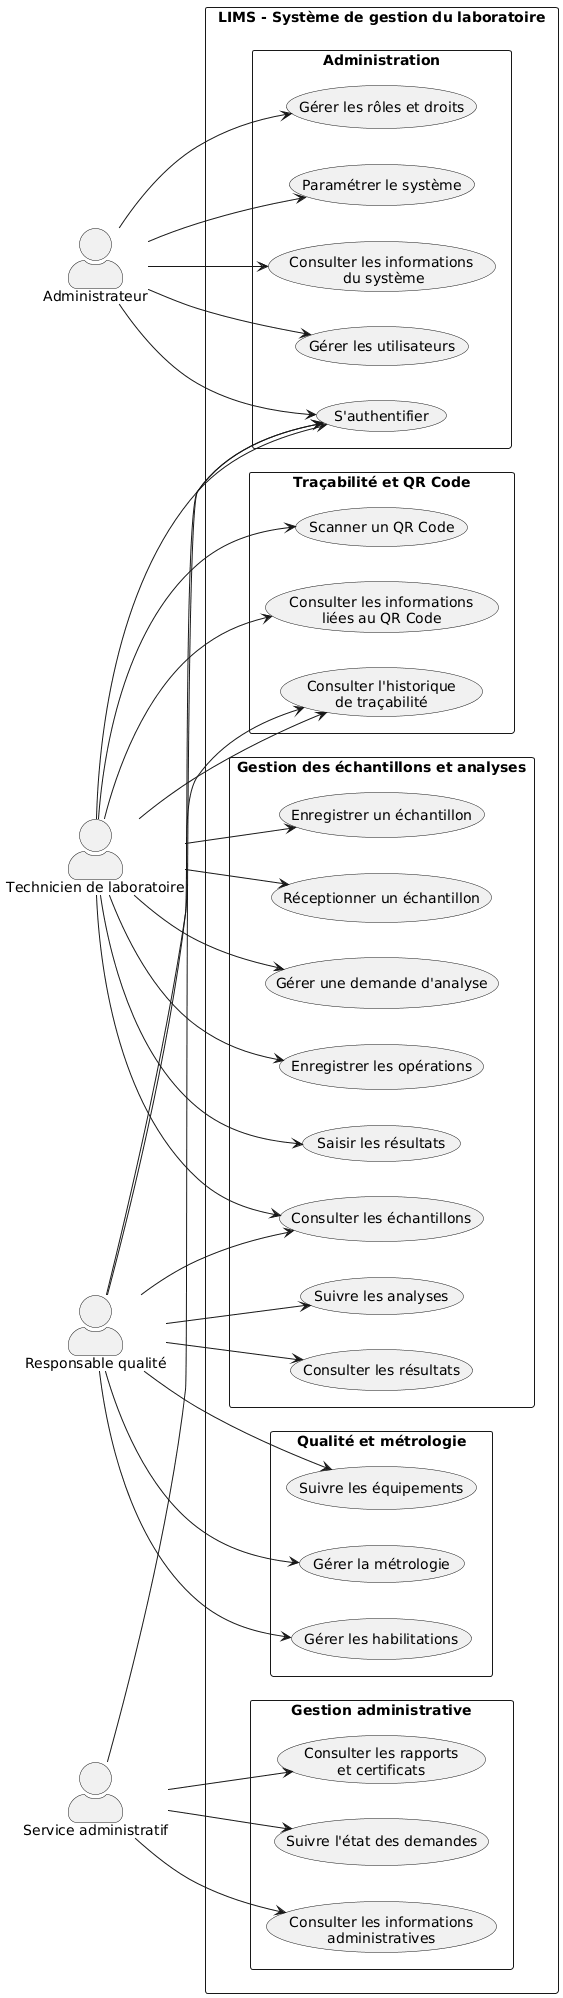
\includegraphics[height=0.78\textheight]{uc-lims.png}
  \caption{Diagramme des cas d'utilisation du LIMS.}
  \label{fig:cas-utilisation}
\end{figure}

\subsection{Diagramme d'activité}

Le diagramme d'activité (figure~\ref{fig:activite-ctaa}) décrit le déroulement global du traitement d'une demande dans le \ac{LIMS}, de l'authentification de l'utilisateur jusqu'à l'archivage des données. Il montre en particulier les deux manières d'identifier un échantillon : par lecture du code \ac{QR}, qui récupère automatiquement les analyses associées, ou par recherche manuelle.

\begin{figure}[H]
  \centering
  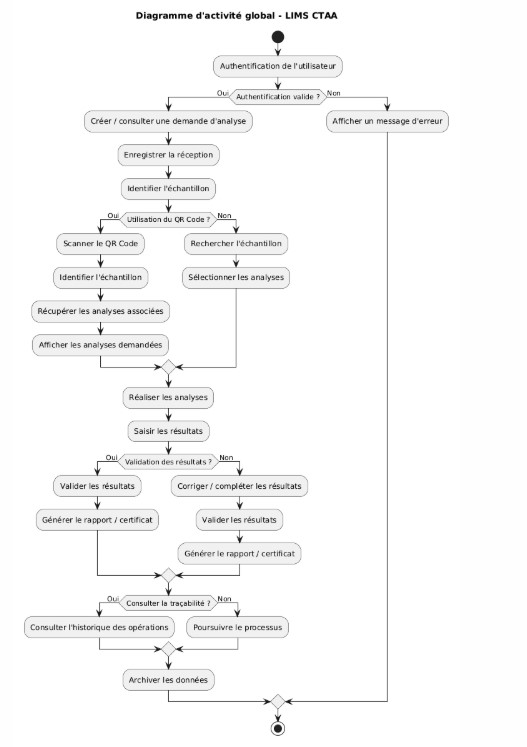
\includegraphics[height=0.72\textheight]{activite-lims.jpg}
  \caption{Diagramme d'activité du traitement d'une demande dans le LIMS.}
  \label{fig:activite-ctaa}
\end{figure}

%-------------------------------------------------------------
\section{Analyse des besoins de Pharmaghreb}
%-------------------------------------------------------------

\subsection{Acteurs}

L'objectif est de récupérer automatiquement les mesures d'un équipement de laboratoire existant, une balance communiquant par liaison série \ac{RS-232}, sans modifier son fonctionnement. Quatre acteurs interagissent avec le module d'acquisition :
\begin{itemize}
    \item \textbf{l'opérateur de laboratoire}, qui s'identifie et réalise les pesées ;
    \item \textbf{l'administrateur technique}, qui installe le module et configure sa connexion réseau ;
    \item \textbf{la balance}, acteur secondaire qui fournit les mesures ;
    \item \textbf{le système d'information} (serveur, application de supervision ou \ac{LIMS}), acteur secondaire qui récupère les données.
\end{itemize}

\subsection{Besoins fonctionnels}
\begin{itemize}
    \item acquérir automatiquement les mesures de la balance, pour supprimer la saisie manuelle ;
    \item identifier l'opérateur par badge \ac{NFC}, afin de rattacher chaque mesure à une personne ;
    \item informer l'opérateur localement de l'état du dispositif (connexion réseau, adresse \ac{IP}, dernière mesure) ;
    \item mettre les mesures à disposition du système d'information via le réseau \ac{Wi-Fi} ;
    \item permettre la configuration du réseau sans reprogrammation, et sa réinitialisation par un bouton.
\end{itemize}

\subsection{Besoins non fonctionnels}
\begin{itemize}
    \item \textbf{Non-intrusivité} : ne modifier ni le matériel ni le paramétrage métrologique de la balance ;
    \item \textbf{Compatibilité électrique} : adapter les niveaux du \ac{RS-232} (jusqu'à $\pm$15~V) aux niveaux logiques 3,3~V du microcontrôleur \citep{tia232} ;
    \item \textbf{Fiabilité des données} : transmettre la valeur exacte affichée par la balance, avec son unité et son état de stabilité ;
    \item \textbf{Faible coût et faible encombrement}, pour pouvoir équiper plusieurs postes ;
    \item \textbf{Évolutivité} : pouvoir connecter d'autres équipements et alimenter à terme un \ac{LIMS}.
\end{itemize}

\subsection{Diagramme des cas d'utilisation}

La figure~\ref{fig:uc-pharmaghreb} présente les cas d'utilisation du module d'acquisition.

\begin{figure}[H]
\centering
\begin{tikzpicture}
  \node[draw=bleu, thick, rounded corners=4pt, minimum width=8.2cm, minimum height=10.6cm,
        label={[font=\small\bfseries, text=bleu]below:Module d'acquisition}] (sys) at (0,0) {};
  \node[cu] (nfc)  at (0, 3.9)  {S'identifier par badge NFC};
  \node[cu] (pes)  at (0, 2.4)  {Effectuer une pesée};
  \node[cu] (acq)  at (0, 0.9)  {Acquérir la mesure};
  \node[cu] (etat) at (0,-0.6)  {Consulter l'état du dispositif};
  \node[cu] (get)  at (0,-2.1)  {Récupérer les mesures};
  \node[cu] (cfg)  at (0,-3.6)  {Configurer le réseau Wi-Fi};

  \bonhomme{(-6.2,2.6)}{Opérateur}
  \bonhomme{(-6.2,-3.0)}{Administrateur\\technique}
  \bonhomme{(6.2,1.5)}{Balance}
  \bonhomme{(6.2,-2.4)}{Système\\d'information}

  \draw[thick, gris] (-5.85,2.8) -- (nfc.west);
  \draw[thick, gris] (-5.85,2.8) -- (pes.west);
  \draw[thick, gris] (-5.85,2.8) -- (etat.west);
  \draw[thick, gris] (-5.85,-2.8) -- (cfg.west);
  \draw[thick, gris] (-5.85,-2.8) -- (etat.west);
  \draw[thick, gris] (5.85,1.7) -- (acq.east);
  \draw[thick, gris] (5.85,-2.2) -- (get.east);
  \draw[fleche, dashed] (pes) -- node[right, etiq] {«include»} (acq);
\end{tikzpicture}
\caption{Diagramme des cas d'utilisation du module d'acquisition (Pharmaghreb).}
\label{fig:uc-pharmaghreb}
\end{figure}

%-------------------------------------------------------------
\section*{Conclusion}
\addcontentsline{toc}{section}{Conclusion}
%-------------------------------------------------------------

Ce chapitre a défini les acteurs et les besoins fonctionnels et non fonctionnels du \ac{LIMS} et de son module de traçabilité, modélisés par des diagrammes de cas d'utilisation et d'activité. Il a ensuite précisé les besoins du module d'acquisition de Pharmaghreb. Le chapitre suivant présente la conception des deux solutions.
